% SPDX-License-Identifier: CC-BY-SA-4.0
% Author: Matthieu Perrin
% Part: 
% Section: 
% Sub-section: 
% Frame: 

\begingroup

\begin{frame}{La loi d'Amdahl}
    \begin{description}
    \item[$p$: ] Proportion du programme parallélisable 
    \item[$T(n)$: ] Temps nécessaire à $n$ threads
    \item[$S(n)$: ] Accélération (Speedup) $S(n) = \frac{T(1)}{T(n)}$ 
    \end{description}
    \pause
    \hspace{\fill}
    \begin{minipage}{.6\textwidth}
    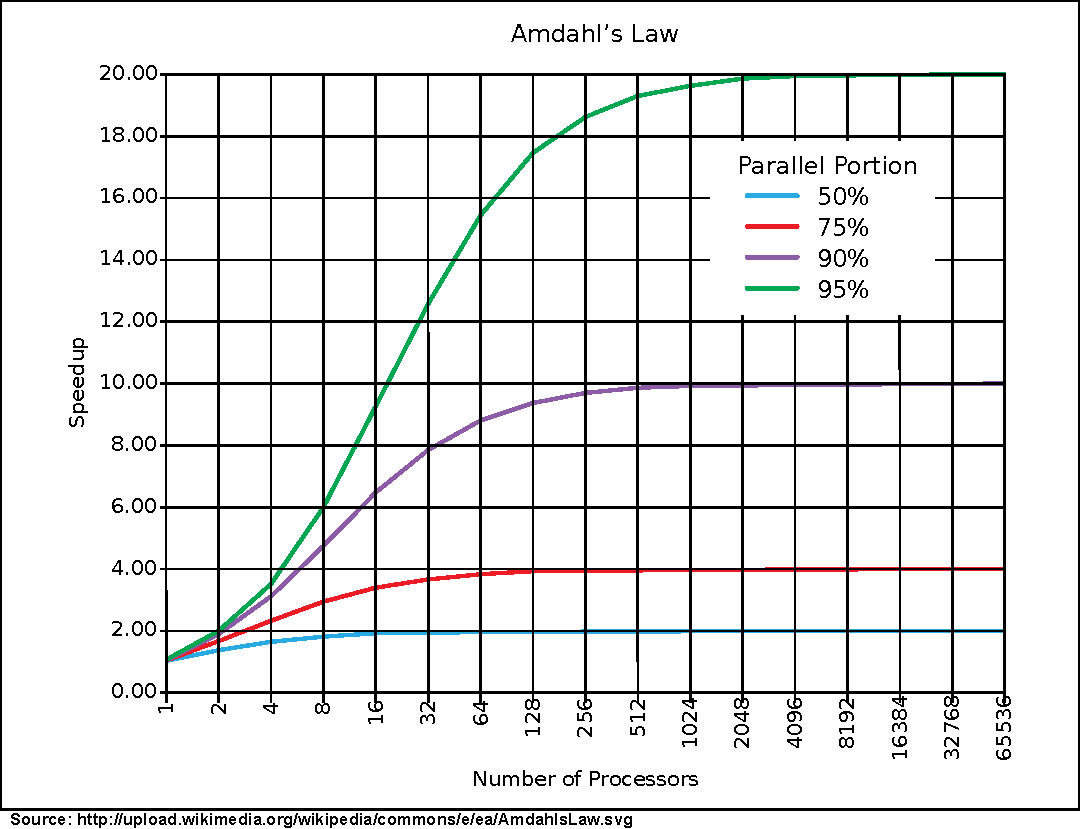
\includegraphics[width=\textwidth]{amdahl-law}
    \end{minipage}
    \hspace{\fill}
    \begin{minipage}{.35\textwidth}
      \vspace{-1cm}
      $$
      \begin{array}{rcl}
        \displaystyle S(n) &\displaystyle =& \displaystyle \frac{1}{1-p + \frac{p}{n}}\\
        \\
        \displaystyle S(n) &\displaystyle <& \displaystyle\frac{1}{1-p}\\
        \\
        \displaystyle \lim_{n\rightarrow \infty} S(n) &\displaystyle =& \displaystyle \frac{1}{1-p}
      \end{array}
      $$
    \end{minipage}
    \hspace{\fill}
\end{frame}

\endgroup
\endinput
